\chapter{Návrh}
\section{Architektura} \label{arch}
V~této kapitole se pokusím navrhnout strukturu jednotlivých komponent výsledného řešení. Celá architektura systému je znázorněna na obrázku \ref{fig:Architecture}. Středobodem systému je server s~nainstalovaným servlet containerem Jetty. V~containeru bude nainstalován Solr. 

Solr bude tvořit backend aplikace. Bude do něj připojena knihovna \emph{Carrot2}, která rozšíří jeho možnosti o~shlukování výsledků, a~má vlastní knihovna s~implementovanými nástroji pro zpracování českého textu pojmenovaná \emph{Analyzery}. Solr bude tedy uchovávat index i~samotný obsah dokumentů, bude zpracovávat vyhledávací dotazy uživatelů a~vracet nalezené výsledky včetně informací o~shlucích a~o~podobnosti dokumentů.

Kromě Solru poběží v~Jetty ještě frontend aplikace. Frontend vytvořím vlastní tak, aby vyhovoval požadavkům. Solr tvoří solidní backend, který komunikuje pomocí HTTP rozhraní a~umožňuje vracet data ve snadno zpracovatelném JSON formátu. Rozhodl jsem se proto, že frontend bude tvořen několika statickými stránkami a~veškerá dynamika bude dodána pomocí JavaScriptu. Stránka se bude pomocí AJAX požadavků dotazovat přímo backendu aplikace --- Solru. Servlety tedy budou jen posílat statické HTML stránky, JavaScriptové knihovny, CSS styly a~podobné soubory. Výhoda řešení spočívá především v jeho jednoduchosti. Celý vyhledávací server bude fungovat v~jednom servlet containeru, vše se tedy zprovozní jen spuštěním nakonfigurovaného Jetty. Zároveň nebudu muset vytvářet stejné rozhraní dvakrát (jednou pro dotazování JavaScriptu webového serveru a~jednou pro dotazování webového serveru Solru).

Poslední komponentou v~architektuře je tzv. Crawler. To bude samostatná aplikace, jejímž úkolem bude indexovat soubory nebo naopak mazat chybějící soubory z~indexu. Připojovat se bude přímo na rozhraní Solru pomocí HTTP. Komunikace se Solrem bude síťová, díky čemuž může aplikace fungovat nejen na stejném stroji s~vyhledávacím serverem, ale i~na jakémkoliv počítači v~síti.

\begin{figure}[h]
\begin{center}
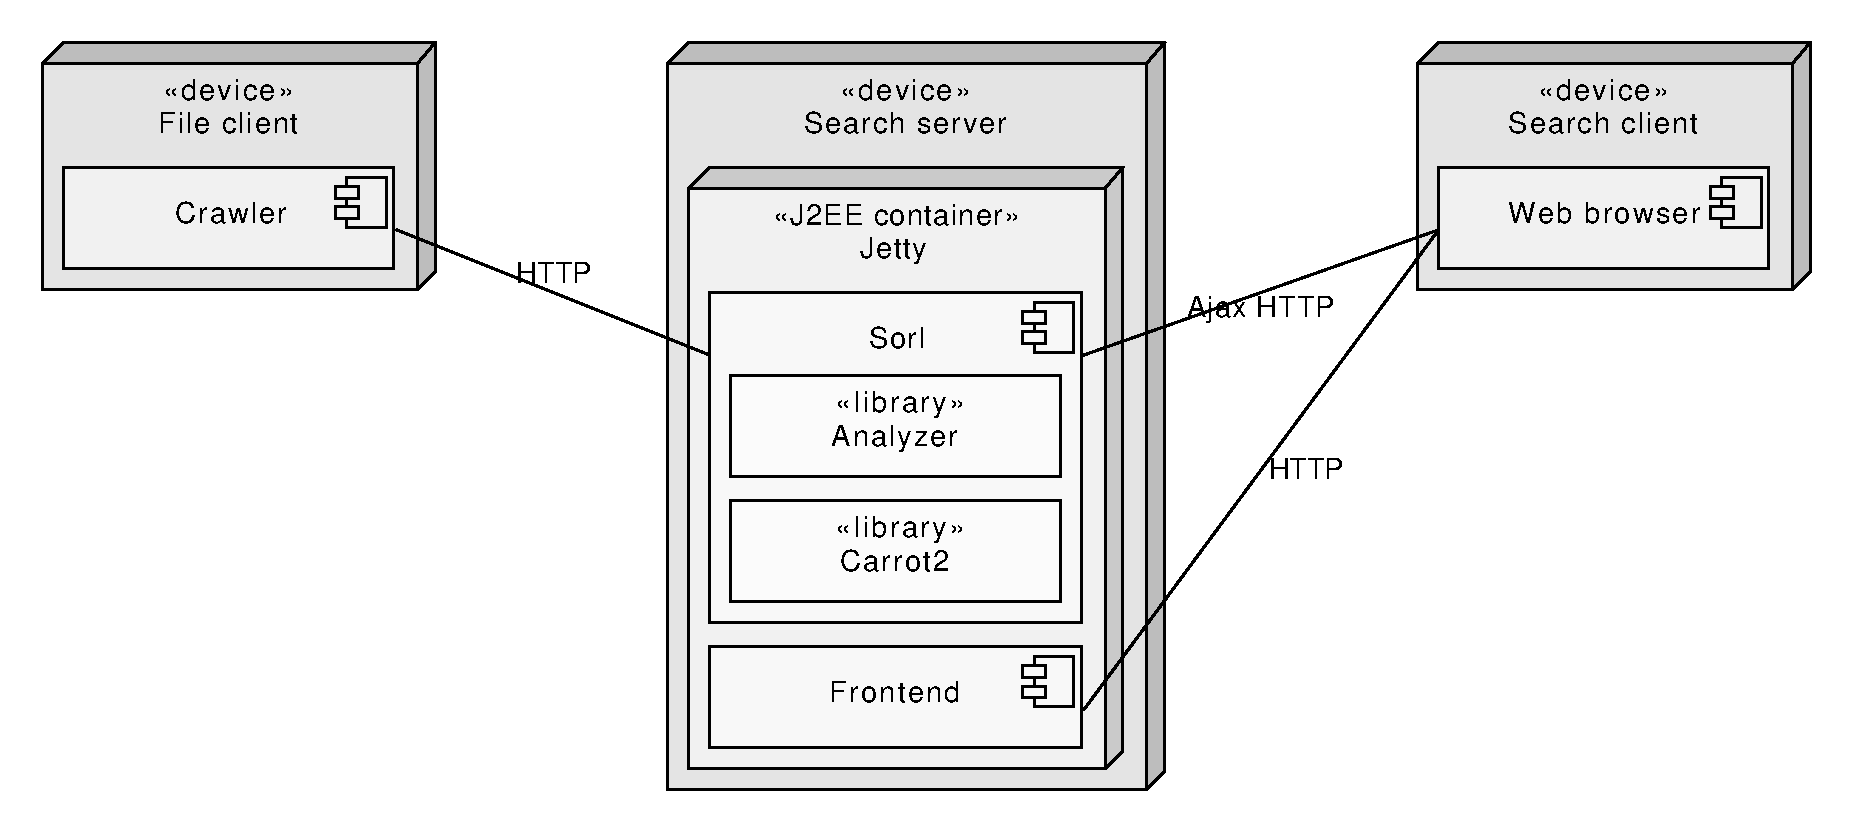
\includegraphics[width=13cm]{Architecture}
\caption{Diagram nasazení}
\label{fig:Architecture}
\end{center}
\end{figure}

\section{Crawler} \label{design_crawler}
Jedná se o~aplikaci, která dle nastavení projde rekurzivně složky file systému, vyhledá všechny soubory, sestaví z~nich Solr dokumenty a~pošle je k~indexaci do Solru. Dále bude procházet dokumenty v~Solru, kontrolovat, zda daný dokument ještě existuje ve filesystému, a~pokud ne, tak jej z~indexu odstraní. Jejím posledním úkolem je kompletní vyprázdnění indexu Solru.

Vzhledem k~tomu, že aplikace bude komunikovat se Solr serverem, rozhodl jsem se, že tuto aplikaci naprogramuji v~jazyce Java, jelikož pro Javu existuje oficiální Java knihovna \emph{Apache SolrJ} pro napojení na Solr server. Kromě této knihovny využiji ještě knihovnu \emph{Apache Log4J} pro zaznamenávání nastalých událostí, která je již závislostí \emph{SolrJ}, a~protože bude součástí aplikace, nebránil jsem se jejímu využití. Konfiguraci programu si usnadním využitím knihovny \emph{Apache commons-configuration}, která mi umožní definovat v~\emph{resources} adresáři výchozí konfigurační hodnoty, které ovšem bude možné přetížit hodnotami jinými pomocí externího konfiguračního souboru nebo pomocí argumentů programu. Díky tomu bude možné měnit chování programu podle aktuálních potřeb.

Aplikaci mám v~plánu navrhnout tak, aby byla rozšiřitelná o~další specializace výše sepsaných úkolů. Zadavetel totiž již během tvorby aplikace předložil několik nových návrhů k~jejímu rozšíření --- například aby aplikace podporovala načítání nejen textových souborů. Existuje také možnost (jak jsem psal v~kapitole \ref{analysis}), že v~budoucnu se bude aplikace napojovat přímo na databázi policejních dokumentů.

\subsection{Návrh tříd}
Během analýzy požadavků jsem nalezl několik společných rysů v~jednotlivých úkolech. Úkol vždy začíná procházením určitého média (např. indexu dokumentů či file systemu). Jednotlivé nalezené prvky (např. Solr dokumenty či soubory) se poté validují (kontroluje se existence na filesystému). V~dalším kroku se prvky parsují či konvertují do jiného datového formátu (soubor na Solr dokument), prvky se pak sbírají do kolekce a~jako kolekce se pak finálně zpracují (pošlou se na server k~zaindexování nebo se smažou z~indexu). Tyto shodné rysy jsem tedy postupně ještě více generalizoval, až jsem nakonec došel k~návrhu, který popisuji níže.

\subsubsection{Procesory}
Jednotlivé úkoly budou prováděny pomocí řetězce procesorů, tříd implementujících rozhraní \emph{IProcessor}.  Procesorové třídy jsou znázorněny v~diagramu \ref{fig:ProcessorClasses}. Řetězec vždy bude začínat \emph{Crawlerem}, tj. třídou, která prochází médium a~předává jednotlivé nalezené prvky prvnímu procesoru v~řetězci. Většina procesorů bude dědit od \emph{AbstractPassThroughProcessor}. Tyto procesory vždy vykonají určitou dílčí činnost a~produkt své činnosti pošlou dalšímu procesoru v~řetězci. Každý procesor bude mít jedinou funkci.

\emph{FactoryProcessor} bude konvertovat data z~jednoho formátu do druhého. Bude tak činit pomocí třídy implementující \emph{IFactory} rozhraní dle návrhového vzoru strategy. Implementovat budu dva typy těchto factory strategií. Jeden typ bude získávat \emph{SolrInputDokument} z~objektu \emph{File} (ten bude použit při indexování dokumentů). Vytvořím dvě implementace: jedna bude umět pouze načítat textové soubory, druhá bude určena pro načítání jakýchkoli textových dokumentů na disku za použití knihovny \emph{Tika}. Druhý typ factory strategie bude z~objektu \emph{SolrDocument} získávat id dokumentu pro kontrolu a~případné smazání z~indexu.

\emph{FilterProcessor} dokáže ze~vstupních dat odfiltrovat některé prvky tím, že je nepředá na výstup. Strategie filtrování bude opět záviset na vložené třídě implementující rozhraní, v~tomto případě rozhraní \emph{IFilter}. Návrh \emph{Factory} a~\emph{Filter} tříd je znázorněn na diagramu \ref{fig:OtherClasses}. Filtry budou použity jen při čištění indexu, všechny tedy souvisí s~tímto úkolem. Do budoucna však nepředstavuje problém rozšířit aplikaci o~filtry souborů. 

Budu implementovat \emph{TrueFilter}, který přijme všechny dokumenty, \emph{NegationFilter}, který bude negovat informaci o~přijetí souboru dalšího vloženého filtru, a~\emph{FileExistsFilter}, který bude kontrolovat existenci souboru. Poslední zmiňovaný filtr bude využívat dříve definované \emph{Factory} pro získání cesty k~souboru ze Sorl dokumentu.

Nakonec bude nutné implementovat \emph{CollectorProcessor}, který sesbírá prvky do kolekce a~nechá je naráz zpracovat dalším procesorem.

Řetězce procesorů budou končit procesorem \emph{IndexingCollectionProcessor} nebo \emph{CleaningCollectionProcessor}. Tyto procesory přijmou kolekci dokumentů k~odstranění či zaindexování a~provedou kýžené změny v~indexu. Komunikace těchto procesorů se Solr serverem bude odstíněna vyčleněním funkcí do samostatné třídy \emph{Index}. \emph{Index} bude pro procesory jednotným modelem pro komunikaci se Solrem a~jeho rozhraní tedy budou procesory používat k~aplikování změn v~indexu.

\begin{figure}[h]
\begin{center}
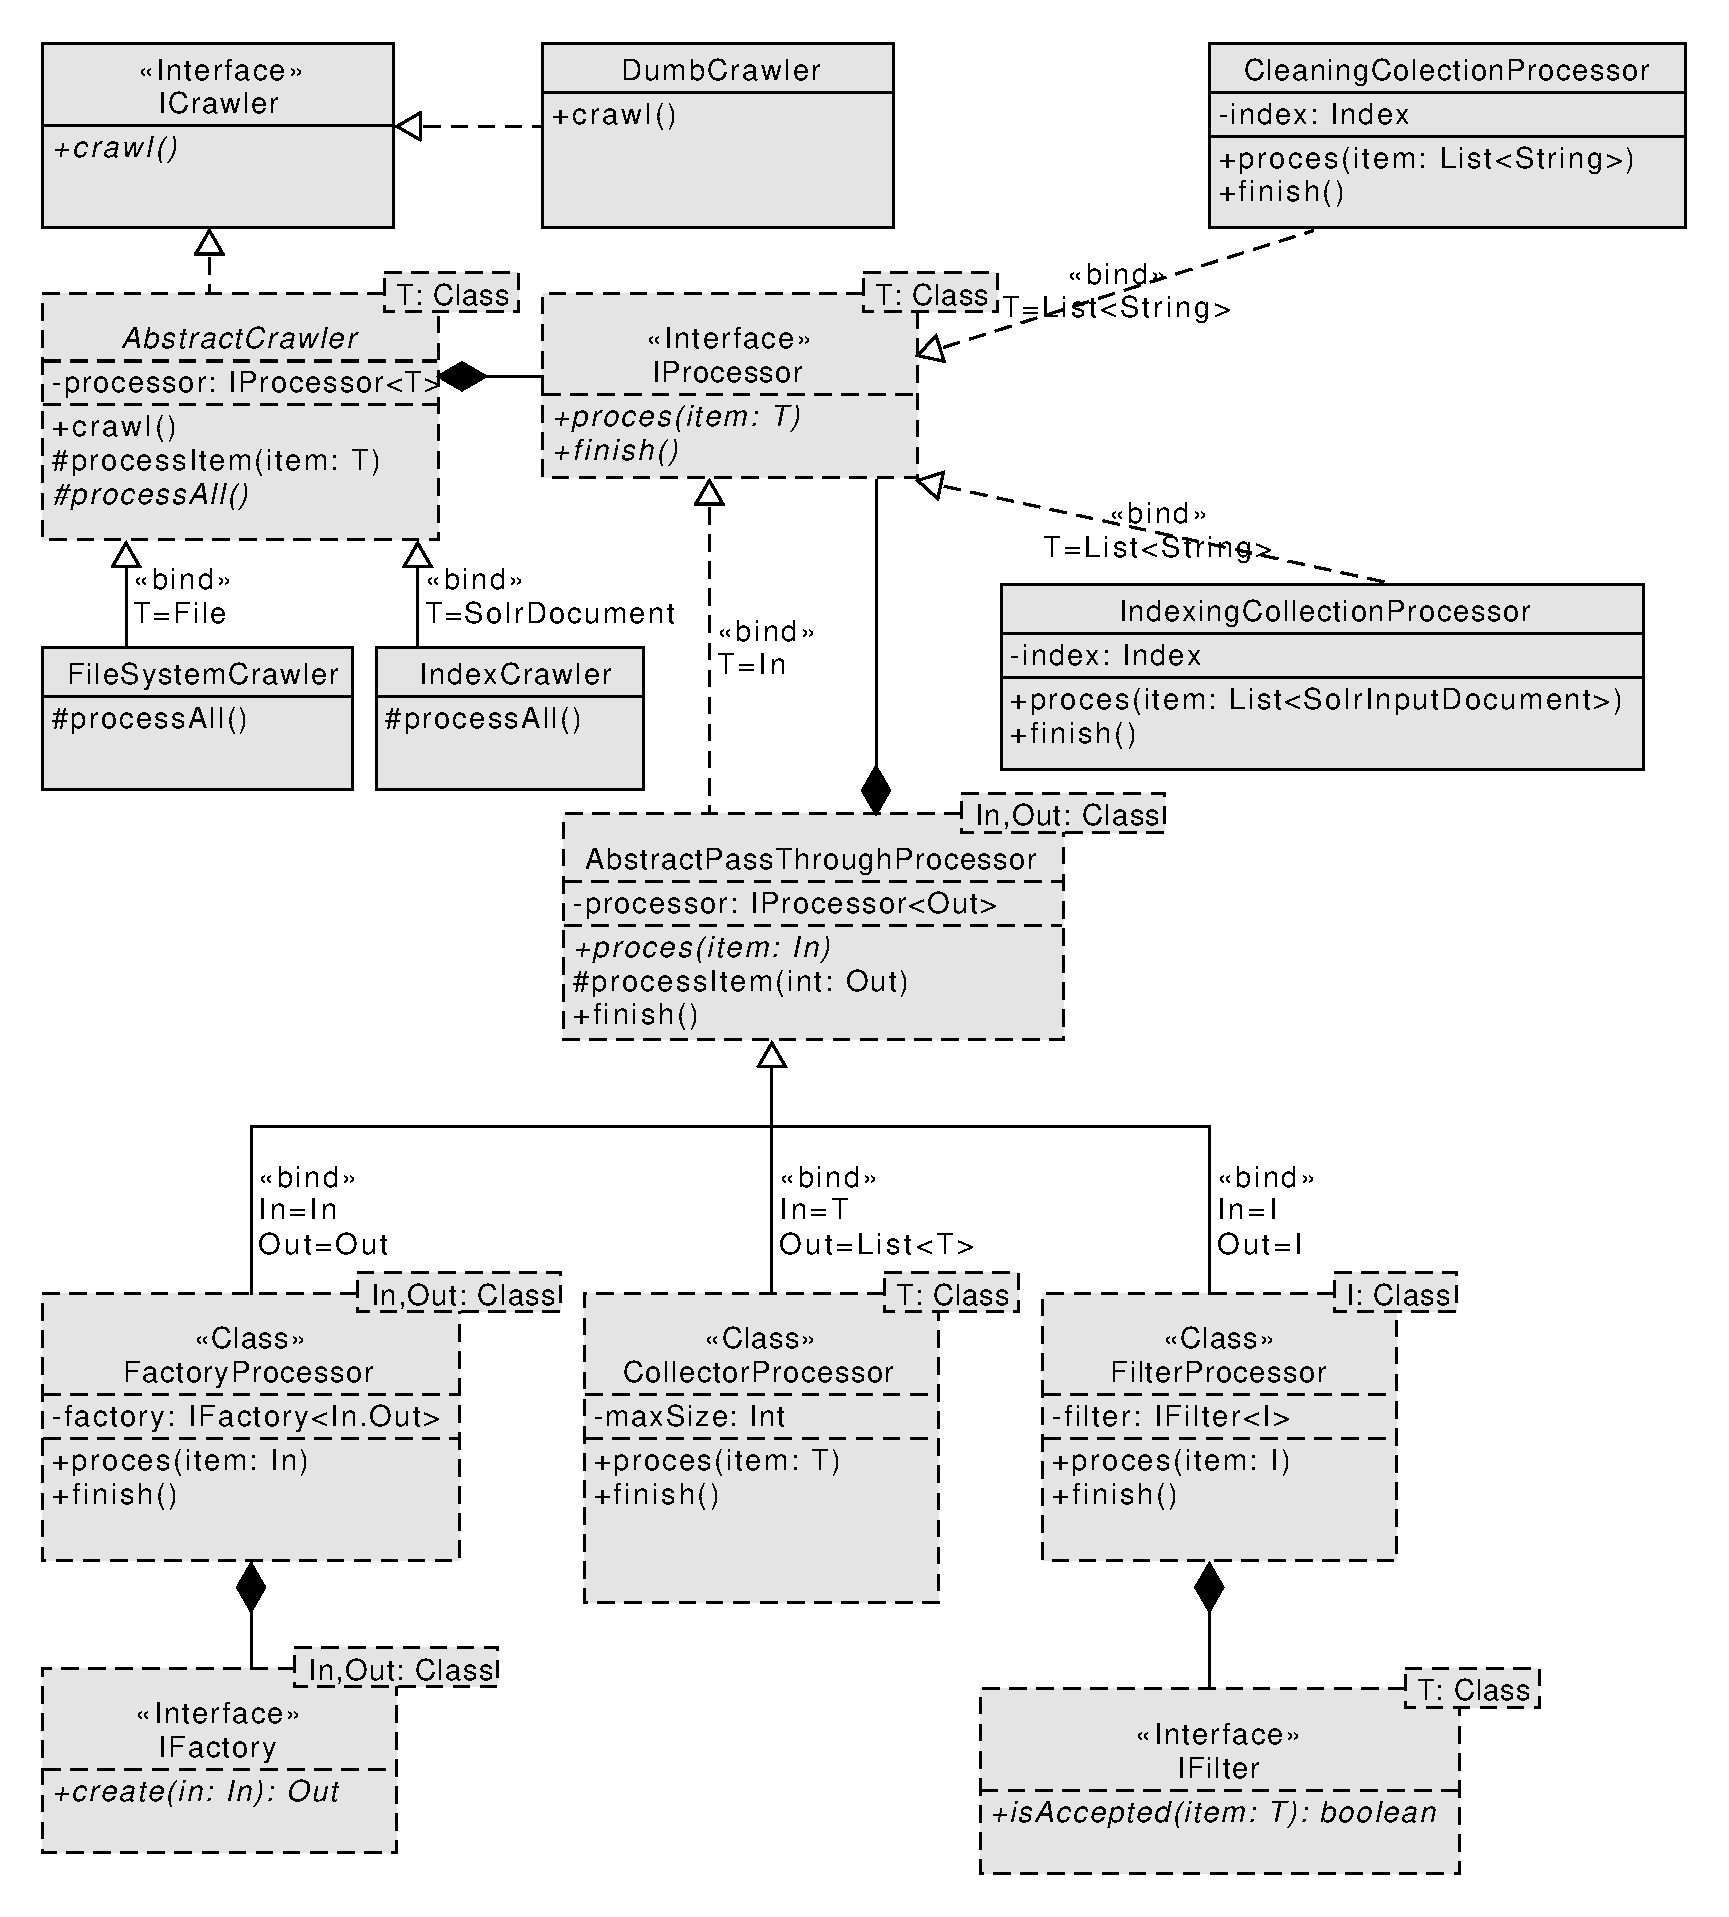
\includegraphics[width=13cm]{ProcessorClasses}
\caption{Diagram procesorových tříd Crawleru}
\label{fig:ProcessorClasses}
\end{center}
\end{figure}

\begin{figure}[h]
\begin{center}
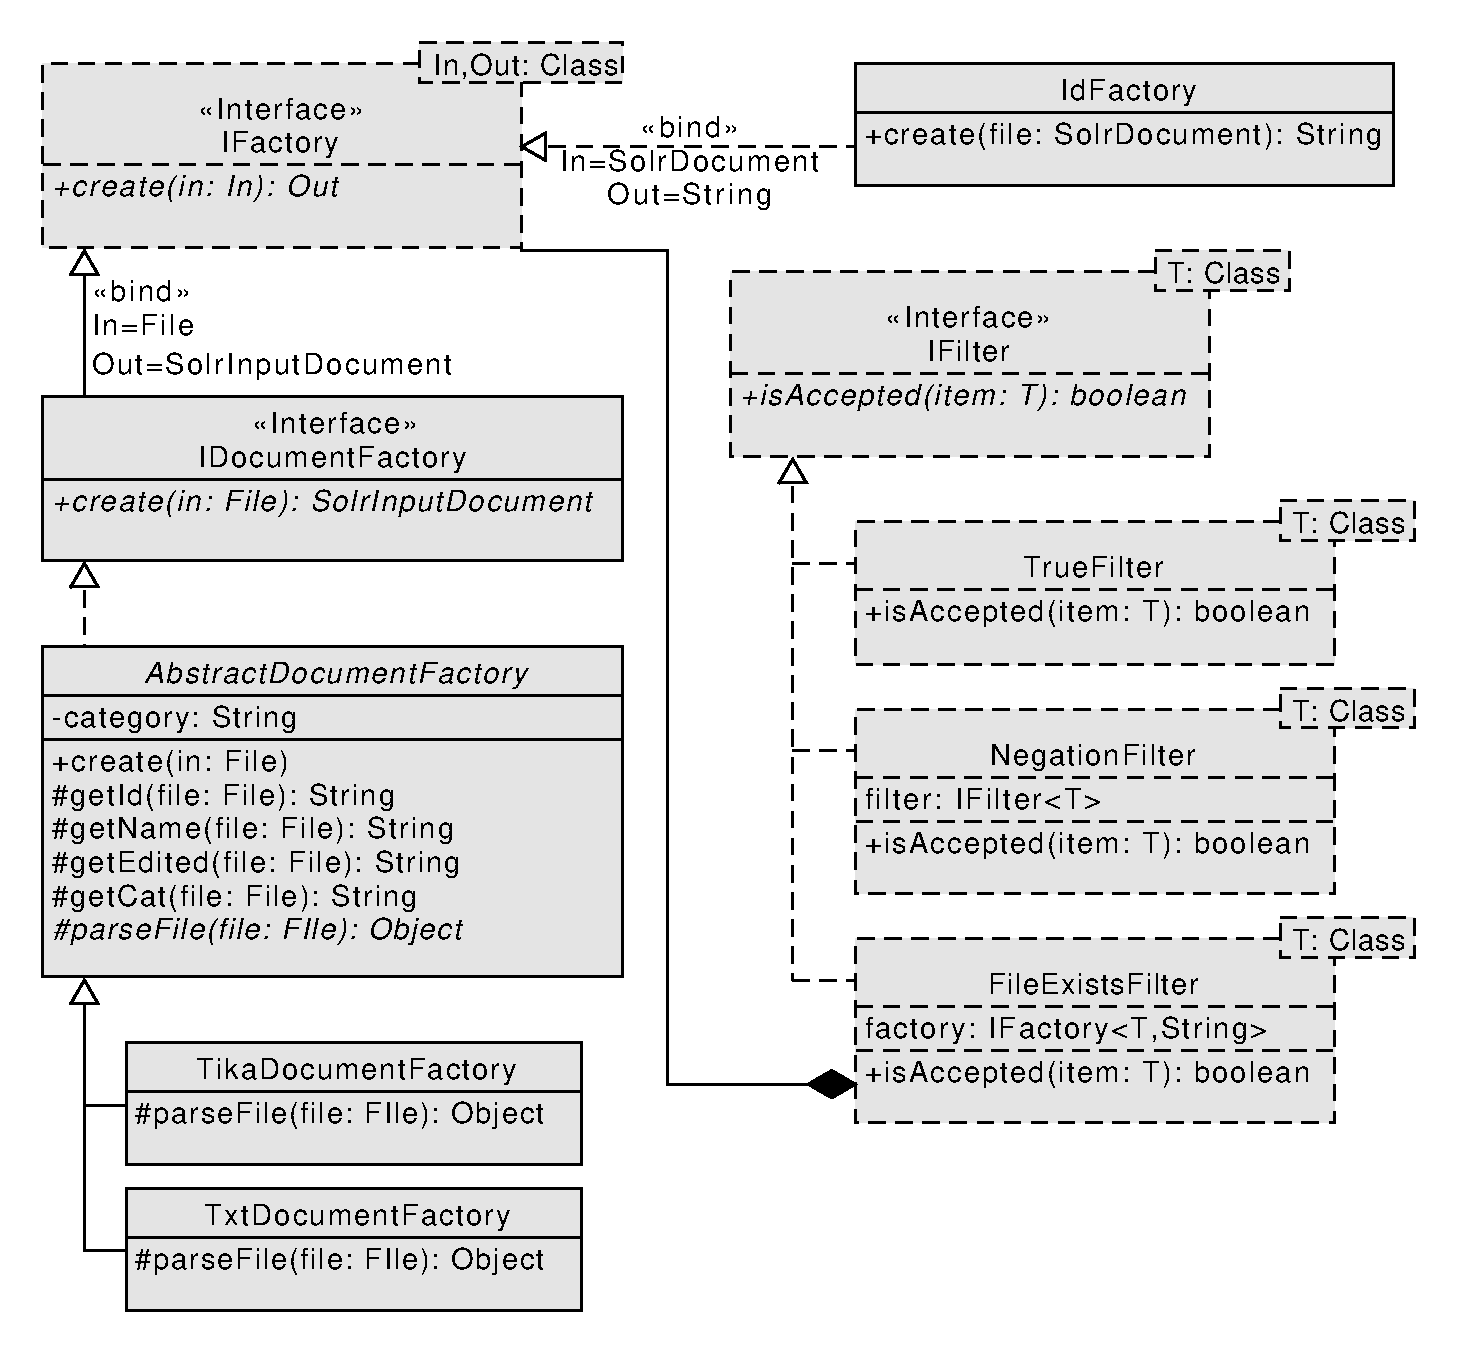
\includegraphics[width=13cm]{OtherClasses}
\caption{Diagram factory a~filter tříd Crawleru}
\label{fig:OtherClasses}
\end{center}
\end{figure}

\subsubsection{Tovární třídy}
Řetězce procesorů budou sestavovány na základě konfigurace, s~využitím návrhového vzoru factory. Sestavování bude mít vždy na starosti daná tovární třída. Tovární třídy se budou řídit parametry přijatými z~konfigurace.

V budoucnosti by bylo možné tyto tovární třídy upravit, aby spolupracovaly s~načítáním tříd a~konfigurací. V~konfiguraci by byl definován řetězec tříd s~případnými konfiguračními parametry. Tovární třída by našla definované třídy (například i~v externích jar knihovnách v~adresáři \emph{lib}), načetla je a~sestavila do řetězce. Tím by byla zaručena absolutní rozšiřitelnost řešení. Podobným způsobem funguje i~konfigurace Solru. Tato verze Crawleru však toto rozšíření zatím obsahovat nebude.

\section{Uživatelské rozhraní} \label{design_frontend}
Na návrhu UI jsem úzce spolupracoval se zadavatelem, abych co nejvíce vyhověl jeho požadavkům. Při návrhu rozhraní jsem se snažil držet se zvyklostí zažitých ve webovém prostředí. Zvláště pak vycházím ze zvyklostí z~internetových vyhledávačů, jako je Google. Další inspirací byl webový frontend aplikace Carrot2. Jelikož jde o~webovou aplikaci, počítá návrh s~proměnnou velikostí okna a~celý layout bude plně responzivní a~přizpůsobitelný pro jakoukoliv velikost okna, včetně mobilní.

Všechny funkční požadavky jde rozdělit do dvou částí: na požadavky týkající se výsledků vyhledávání jako celku (vyhledávání, shlukování) a~požadavky týkající se jednoho vybraného dokumentu (podobnostní vyhledávání, zobrazení obsahu). Uživatelské rozhraní tedy bude sestávat také ze dvou layoutů, z nichž každý bude odpovídat jedné skupině požadavků. Mezi layouty se pak bude volně procházet proklikem. 

Layouty budou mít společný jednotící prvek, a~to hlavičku stránky s~logem aplikace, které bude umístěné tradičně v~levém horním rohu stránky. Zbytek hlavičky bude odpovídat kontextu daného layoutu, aby se neplýtvalo místem. Hlavička bude i~nositelem informace o~kontextu aktuální stránky a~bude napovídat, v~jaké části se uživatel nachází.

\subsection{Vyhledávání dokumentů}
Výchozí stránka bude mít v~hlavičce vyhledávací formulář. Layout je znázorněn na obrázku \ref{fig:SearchLayout}. Formulář bude obsahovat vstupní pole pro výběr zdroje v~podobě roletky, kde uživatel zvolí, který index dokumentů se má pro vyhledávání použít. V~roletce by měl být automaticky vybrán výchozí index nastavený v~Solru. Vpravo od roletky umístím samotné vyhledávací pole a~potvrzovací tlačítko pro vyvolání akce vyhledávání. Vyhledávací pole by mělo být rozměrné a~mělo by vyplnit celou zbývající šířku okna.

\begin{figure}[h]
\begin{center}
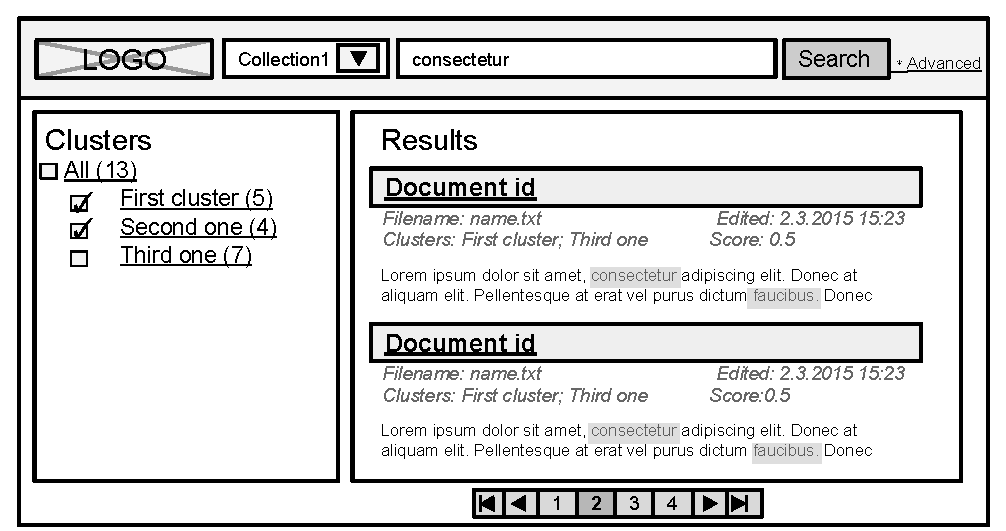
\includegraphics[width=13cm]{SearchLayout}
\caption{Návrh vyhledávacího uživatelského rozhraní}
\label{fig:SearchLayout}
\end{center}
\end{figure}

Vpravo od potvrzovacího tlačítka bude dále umístěn malý odkaz se šipkou, který bude přepínat zobrazení rozšířené nabídky nastavení vyhledávání. Podobu rozšířené nabídky můžeme pozorovat na obrázku \ref{fig:AdvancedLayout}. Nabídka bude stále ještě součástí hlavičky stránky (hlavička se o~ní vlastně rozšíří). Měla by obsahovat jen roletku pro přepínání shlukovacího algoritmu, v~budoucnu bude možné přidat další volby.

\begin{figure}[h]
\begin{center}
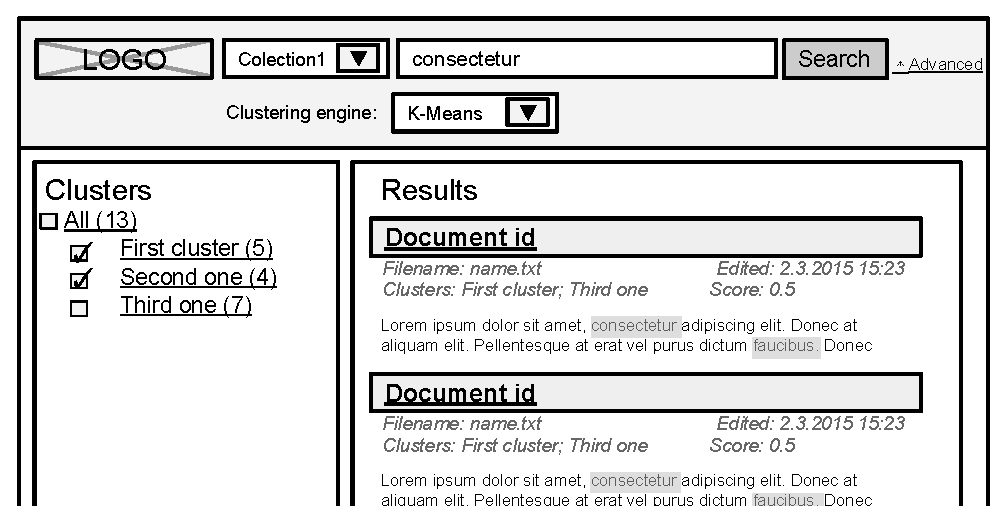
\includegraphics[width=13cm]{AdvancedLayout}
\caption{Návrh vyhledávacího uživatelského rozhraní s~rozšířenou nabídkou}
\label{fig:AdvancedLayout}
\end{center}
\end{figure}

Pod hlavičkou se zobrazí samotný vyhledaný obsah. Všechen vyhledaný obsah projde rovnou shlukovací analýzou. Shlukování nebude nutné zapínat. Vlevo bude umístěn sloupec o~šířce rovné čtvrtině šířky okna s~nalezenými shluky. Vpravo se pak ve zbývající šířce zobrazí nalezené výsledky. Pokud bude okno příliš úzké, zobrazí se výsledky až pod seznamem shluků a~shluky i~výsledky se roztáhnou na plnou šíři okna.

Sloupec se shluky bude mít formu odrážkového seznamu. Nejvyšší prvek seznamu je shluk \uv{All}, který bude obsahovat všechny nalezené výsledky. Pod ním teprve budou jednotlivé nalezené shluky. U~každého shluku se zobrazí číslo odpovídající počtu obsažených dokumentů. Seznam shluků bude provádět i~filtrování dokumentů. Kliknutím na shluk se shluk označí (v obrázku \ref{fig:SearchLayout} je označen zatržítkem) a~ve výsledcích se zobrazí jen dokumenty patřící do vybraného shluku. Vybrat takto půjde libovolný počet shluků. Při každém novém hledání se vždy jako výchozí označí shluk \uv{All}, aby se zobrazily ve výsledcích všechny nalezené dokumenty a~teprve sám uživatel si provedl případnou filtraci.

Sloupec s~výsledky bude obsahovat nalezené dokumenty ve vybraných shlucích. Každý dokument bude reprezentován svým ID v~podobě odkazu vedoucího na zobrazení obsahu dokumentu. Pod ID budou zobrazena různá metadata, jako jméno souboru, kdy byl dokument naposledy upraven, skóre (tj. číslo vyjadřující míru shody hledaného výsledku s~hledaným výrazem) či seznam clusterů, do kterých dokument patří. Pod metadaty bude umístěn úryvek obsahu dokumentu se zvýrazněnými hledanými výrazy. Výsledky budou řazeny podle skóre.

Na konci stránky pod výsledky bude umístěno ovládání stránkování: tlačítka pro posun na předchozí či další stránku, na první či poslední stránku a~seznam několika stránek v~okolí aktuálně zobrazené stránky, která bude na tomto panelu zvýrazněna.

Pořadí sloupců se shluky a~s~výsledky jsem volil s~ohledem na posloupnost pracovního postupu a~na zvyklosti. Lze předpokládat, že uživatel po zadání dotazu nejdříve prohlédne shluky a~vybere, z~kterých shluků chce dokumenty vidět. Seznam shluků má zároveň funkčně nejblíže k~menu, a~to je zvykem na internetových stránkách umisťovat po levé straně od obsahu.

\subsection{Detail dokumentu}
Kliknutím na ID dokumentu ve výsledcích vyhledávání se dostaneme do zobrazení detailu dokumentu. Návrh stránky je znázorněn na obrázku \ref{fig:DetailLayout}. Layout této stránky bude mít v~hlavičce kromě loga už jen vypsané ID otevřeného dokumentu a~bude opět dvousloupcový. Vlevo bude umístěn obsah samotného dokumentu, vpravo sloupec o~šířce jedné třetiny šířky okna obsahující seznam podobných dokumentů k~aktuálně zobrazenému. Bude-li okno příliš malé, sloupce se zobrazí pod sebou na plné šíři okna, stejně jako u~vyhledávacího layoutu. Pořadí sloupců je opět dáno zvyklostmi na internetových stránkách. Sloupec s~podobnými dokumenty se obvykle spolu s~dalšími kontextovými informacemi umisťuje  do pravého sloupce vedle hlavního obsahu, případně pod obsah.

Sloupec s~obsahem bude ve vrchní části zobrazovat metadata dokumentu a~následovat bude celý text dokumentu. Vyhledávané fráze budou v~textu zvýrazněny.

Pravý sloupec bude obsahovat seznam dokumentů, které jsou podobné dokumentu právě otevřenému. Seznam bude strukturován podobně jako seznam výsledků ve vyhledávacím layoutu: bude obsahovat ID dokumentu, které bude zároveň odkazem na detail příslušného dokumentu, poté budou následovat metadata dokumentu a~úryvek obsahu. Dokumenty budou v~tomto sloupci řazeny podle skóre, které vyjadřuje míru podobnosti dokumentu s~otevřeným dokumentem.

\begin{figure}[h]
\begin{center}
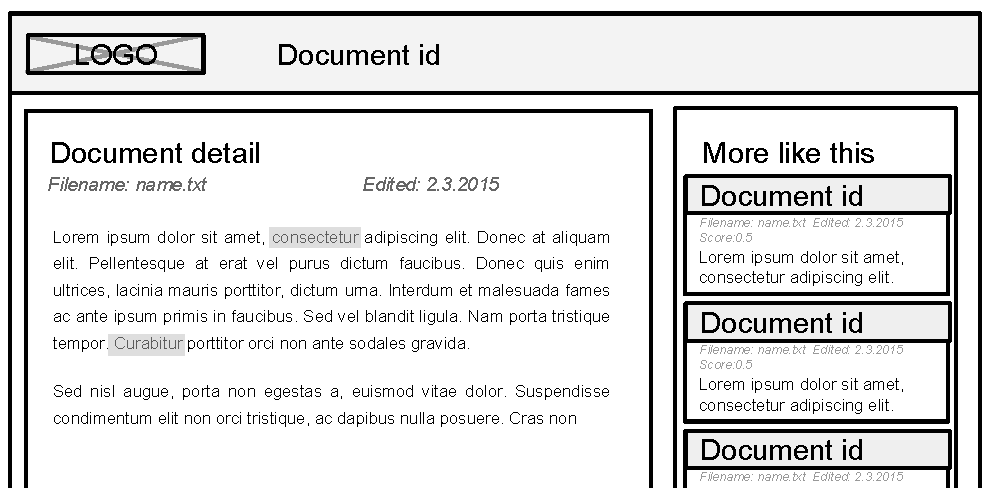
\includegraphics[width=13cm]{DetailLayout}
\caption{Návrh uživatelského rozhraní pro zobrazení dokumentu}
\label{fig:DetailLayout}
\end{center}
\end{figure}